% =================================================================
% Codice LaTeX per importare i tre grafici della tesi in Overleaf.
%
% Copia i tre PDF (fig_robustezza_proxy.pdf, fig_qe_bande.pdf,
% fig_identificazione.pdf) nella stessa cartella del .tex di Overleaf
% (es. "figure/"), poi includi nel testo i blocchi sottostanti.
%
% Dipendenze nel preambolo:
%   \usepackage{graphicx}
%   \usepackage{booktabs}   % facoltativo (non usato qui)
%   \usepackage{amsmath, amssymb}   % per simboli matematici nelle caption
%
% Bozze di caption inserite: la formulazione finale, in particolare le
% sfumature di onestà su robustezza e identificazione, è di Francesco.
% =================================================================


% ---------------------- FIGURA 1 -----------------------------------
% Robustezza del coefficiente strutturale alla costruzione della componente
% di tasso del bond.

\begin{figure}[t]
    \centering
    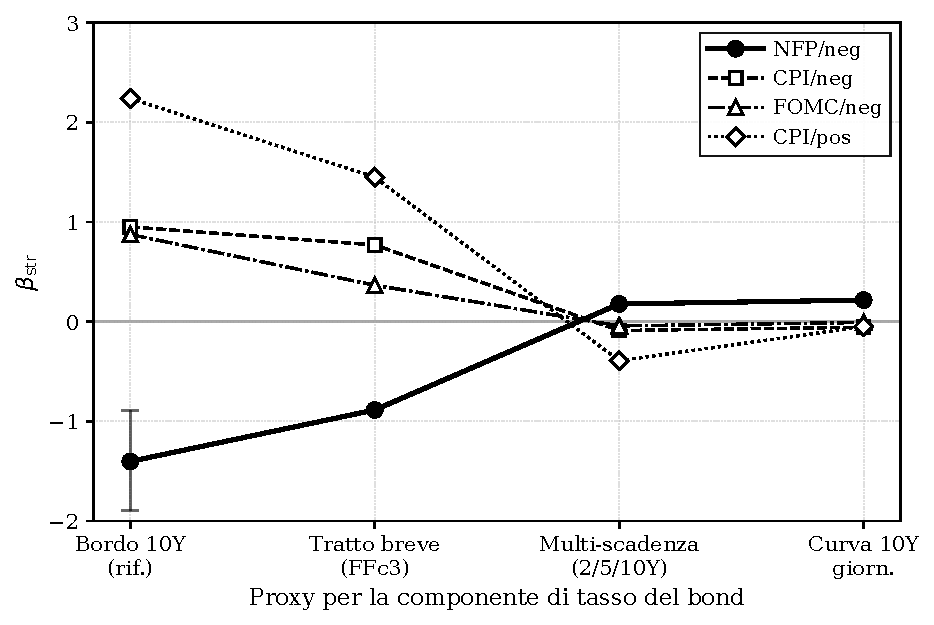
\includegraphics[width=0.85\linewidth]{figure/fig_robustezza_proxy.pdf}
    \caption[Robustezza di $\beta_{\mathrm{str}}$ alla proxy della componente
             di tasso]{Coefficiente strutturale $\beta_{\mathrm{str}}$ per le
             quattro celle identificate dal cancello del pacchetto
             \texttt{decomposition}, al variare della proxy con cui si
             costruisce la componente di tasso $\Delta P^{B}_{b}$. Asse $x$:
             le quattro costruzioni della proxy, in ordine il bordo $10$Y
             del riferimento autoritativo (run del $23$ giugno $2026$,
             $\Delta y_{b} = \Delta\,\mathrm{FFc3}$, $D_{\mathrm{bond}}=8.97$),
             la stessa proxy del tratto breve in un secondo run di confronto,
             la combinazione multi-scadenza $2$--$5$--$10$ con pesi $D_{n}$, e
             la curva $10$Y daily diretta ($\Delta\,\mathrm{DGS10}$). La cella
             \texttt{NFP/neg} (cerchio pieno, linea continua) conserva segno e
             magnitudine sotto le tre proxy intraday-coerenti; le altre tre
             celle attraversano lo zero alla proxy multi-scadenza o alla
             curva $10$Y daily. La barra di errore sul primo punto è la
             banda di sampling al $95\%$ del bootstrap clusterizzato del
             baseline. Asse $y$: $\beta_{\mathrm{str}}$ adimensionale; la
             linea grigia a $y=0$ marca il cambio di segno.}
    \label{fig:robustezza_proxy}
\end{figure}


% ---------------------- FIGURA 2 -----------------------------------
% Trasmissione QE lungo la curva Bund con bande di confidenza.

\begin{figure}[t]
    \centering
    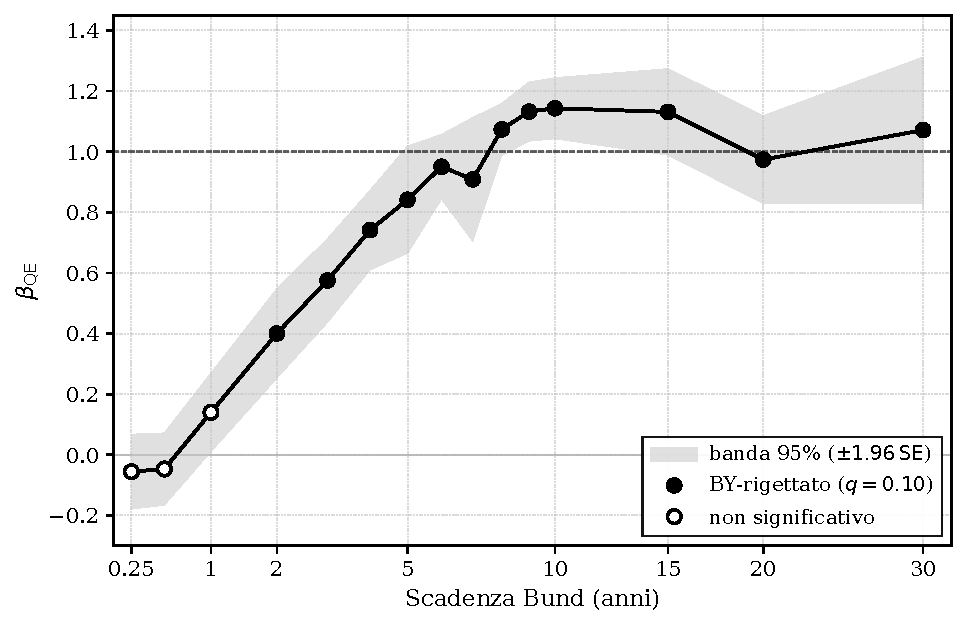
\includegraphics[width=0.88\linewidth]{figure/fig_qe_bande.pdf}
    \caption[Trasmissione del fattore $\mathrm{QE}$ lungo la curva Bund]{
             Coefficiente $\beta_{\mathrm{QE}}$ della trasmissione del fattore
             $\mathrm{QE}$ di Altavilla et al.\ ($2019$) lungo la curva Bund
             a $15$ scadenze, dal $3$ mesi al $30$ anni. Linea nera
             continua: stima $\widehat{\beta}_{\mathrm{QE},n}$ per scadenza
             $n$; banda grigia: $\widehat{\beta}\pm 1.96\,\mathrm{SE}$,
             errori standard HC1. Marcatori pieni: scadenze che superano
             il controllo Benjamini--Yekutieli a $q=0.10$ con $m=15$
             ipotesi ($12$ scadenze su $15$). Marcatori vuoti: scadenze
             non significative dopo correzione. Linea tratteggiata a
             $y=1$: livello di riferimento dell'unità di trasmissione.
             Eventi $n=129$ (post-$2010$ con fattori $\mathrm{T/P/QE}$
             tutti disponibili). Asse $x$ in scala radice per leggibilità
             contemporanea del tratto corto e lungo.}
    \label{fig:qe_bande}
\end{figure}


% ---------------------- FIGURA 3 -----------------------------------
% Meccanismo di identificazione per eteroschedasticita'.

\begin{figure}[t]
    \centering
    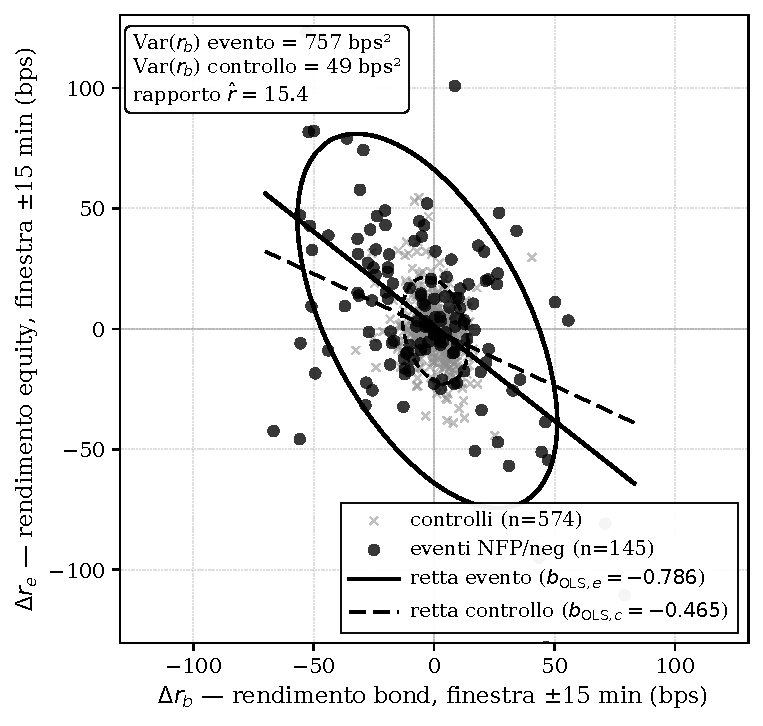
\includegraphics[width=0.72\linewidth]{figure/fig_identificazione.pdf}
    \caption[Identificazione per eteroschedasticit\`a sulla cella
             \texttt{NFP/neg}]{Diagramma di dispersione dei rendimenti
             equity--bond nelle finestre di evento (cerchi pieni,
             $n=145$) e nelle finestre di controllo associate (croci
             grigie, $n=574$) per la cella \texttt{NFP/neg}, finestra
             $\pm 15$ minuti. Ellissi di covarianza al livello $95\%$
             (eventi continua, controlli tratteggiata) e rette di
             regressione $\mathrm{OLS}$: pendenza evento
             $b_{\mathrm{OLS},e}=-0.786$, pendenza controllo
             $b_{\mathrm{OLS},c}=-0.465$. La differenza di pendenza
             $b_{\mathrm{OLS},e}-b_{\mathrm{OLS},c}=-0.321$ contro un
             rapporto di varianze del bond $\hat r=15.4$ \`e la firma
             dell'identificazione di Rigobon e Sack: lo stesso fattore
             comune produce dispersione molto pi\`u ampia nelle finestre
             di evento, e da quel salto di dispersione si ricava
             $\widehat\beta_H=-0.808$ ($\mathrm{SE}_{\mathrm{boot}}=0.162$)
             come $\Delta\,\mathrm{Cov}/\Delta\,\mathrm{Var}$ con un test
             $F$-efficace di $53.1$.}
    \label{fig:identificazione}
\end{figure}


% =================================================================
% Avviso d'uso (NON inserire nel PDF finale):
%   - Posizionamento `[t]` di default; spostare a `[h!]` o `[!htbp]` se
%     necessario per il flusso del testo.
%   - Le tre figure sono pensate per essere su una pagina dedicata o
%     all'inizio della relativa sezione del capitolo Risultati.
%   - Le caption sono BOZZE TECNICHE: contengono i numeri e i riferimenti
%     dei pacchetti, ma il fraseggio finale spetta a Francesco, soprattutto
%     per le sfumature di onestà su robustezza condizionale alla proxy
%     (Figura 1) e su predittività vs identificazione (non discussa nei
%     grafici ma rilevante per il capitolo).
% =================================================================
